% ClearEval -- IEEE BIBM submission (converted from the MICCAI 2026 LNCS manuscript)
% Two-column IEEE conference format (IEEEtran). Content maps the MICCAI
% manuscript section-by-section; structure/numbers/claims are preserved.
% Compile: pdflatex main -> bibtex main -> pdflatex main -> pdflatex main

\documentclass[conference]{IEEEtran}
\IEEEoverridecommandlockouts
% The preceding line is only needed to identify funding in the first footnote.
% If that is unneeded, please comment it out.

\usepackage{cite}
\usepackage{amsmath,amssymb,amsfonts}
\usepackage{graphicx}
\usepackage{booktabs}
\usepackage{multirow}
\usepackage{textcomp}
\usepackage{xcolor}
\usepackage[T1]{fontenc}
\usepackage{url}
\usepackage{tabularx}
\usepackage{booktabs}
\usepackage{tabularx}


\begin{document}

\title{ClearEval: A Database-Grounded Feasibility Benchmark for LLM-Generated Tissue Optical Clearing Protocols}

% ---------------------------------------------------------------------------
% NOTE: IEEE BIBM uses double-blind review. The author block below is
% anonymized to mirror the MICCAI submission. For the camera-ready version,
% delete the anonymized block and uncomment the six-author IEEE template.
% ---------------------------------------------------------------------------
\author{\IEEEauthorblockN{Anonymous Author(s)}
\IEEEauthorblockA{\textit{Affiliation withheld for double-blind review} \\
email withheld}}

% --- Camera-ready author template (IEEEtran supports up to six authors) ---
% \author{\IEEEauthorblockN{1\textsuperscript{st} Given Name Surname}
% \IEEEauthorblockA{\textit{dept. name of organization (of Aff.)} \\
% \textit{name of organization (of Aff.)}\\
% City, Country \\
% email address or ORCID}
% \and
% \IEEEauthorblockN{2\textsuperscript{nd} Given Name Surname}
% \IEEEauthorblockA{\textit{dept. name of organization (of Aff.)} \\
% \textit{name of organization (of Aff.)}\\
% City, Country \\
% email address or ORCID}
% }

\maketitle

\begin{abstract}
Tissue Optical Clearing (TOC) enables non-destructive, high-resolution 3D imaging, but designing a feasible protocol requires aligning the experimental goal, specimen type, and fluorescence/labeling modality with an appropriate clearing method and protocol parameters. Existing biomedical LLM evaluations have emphasized static knowledge, question answering, and text-based reasoning, while the experimental feasibility of generated wet-lab protocols remains less studied. We introduce ClearEval, a database-grounded, text-reference-free feasibility benchmark for LLM-generated TOC protocols. ClearEval is built on a structured TOC feasibility database integrating 372 wet-lab experimental records, 400+ curated tissue-clearing literature chunks, and expert-reviewed constraints on methods, tissues, markers, timing, and compatibility. It contains 253 open-ended protocol-generation scenarios for evaluating TOC protocols, plus a 2{,}588-question static knowledge audit to separate knowledge gaps from application failures. Generated protocols are evaluated with CCE, a three-part framework covering Completeness, Correctness, and Effectiveness. Completeness and Correctness are scored by LLM-based rubric judgment, while Effectiveness is computed from database-grounded feasibility rules and formulas. Applying ClearEval to 13 state-of-the-art LLMs, we find that static TOC knowledge does not reliably translate into feasible protocol generation. The dominant failures arise from executable parameterization in TOC, especially matching fluorescent markers to required labeling targets. ClearEval converts expert criteria for TOC protocol feasibility into a computable evaluation framework. It provides a depth-first feasibility benchmark for TOC and a re-curatable template for building similar benchmarks in other wet-lab domains. Code and data:
\url{https://anonymous.4open.science/r/ClearEval}.

\end{abstract}

\begin{IEEEkeywords}
Benchmark, Tissue optical clearing, Wet-lab protocols, Large language models
\end{IEEEkeywords}

\section{Introduction}

\begin{figure*}[t]
\centering
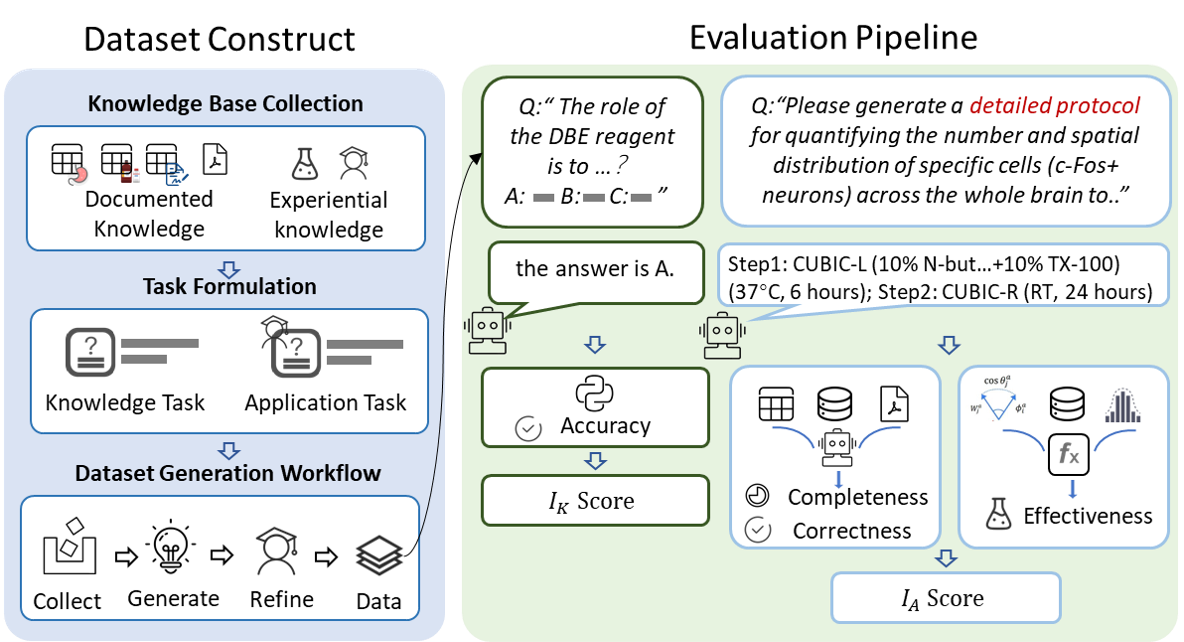
\includegraphics[width=0.8\textwidth]{figures/overview.png}
\caption{Overview of ClearEval. A TOC feasibility database is constructed
from wet-lab experimental records, curated literature chunks, and
expert-reviewed constraints. The database supports both task construction
and protocol scoring. The Knowledge track is scored by the Knowledge Index
($I_K$), while the Application track is scored by the Application Index
($I_A$), which combines Completeness, Correctness, and Effectiveness.}
\label{fig:overview}
\end{figure*}

Tissue Optical Clearing (TOC) renders biological tissues optically transparent
by reducing light scattering and refractive-index mismatch, enabling
non-destructive, high-resolution 3D imaging via light-sheet
microscopy~\cite{ueda2020tissue,chung2013clarity}. However, designing a TOC
protocol is not a single-answer task. Given a specimen, labeling target,
imaging goal, and laboratory constraint, experimenters must choose a feasible
combination of clearing method, labeling strategy, refractive-index condition,
incubation schedule, sample geometry, and operational constraints. Multiple
combinations may be acceptable, but one incompatibility---for example, a
quenched fluorophore, an unsuitable method for the sample scale, or an
unrealistic incubation time---can invalidate the protocol and irreversibly
damage the specimen.

Existing biomedical LLM benchmarks, including MedQA~\cite{jin2021disease},
MMLU~\cite{hendrycks2021mmlu}, and recent biomedical
extensions~\cite{zhang2025benchmarking,wang2025cardbiomedbench,feng2024mediq},
have advanced the evaluation of biomedical knowledge, question answering, and
text-based reasoning. For generated wet-lab protocols, the key question is not only textual plausibility, but alignment with real experimental constraints. Likewise, semantic metrics such as
BLEU~\cite{papineni2002bleu} and general-purpose LLM
evaluators~\cite{liu2023geval,li2024survey} do not explicitly evaluate
method--label compatibility, refractive-index suitability, or timing
plausibility. This creates a gap between knowledge evaluation and
pre-experimental feasibility checking.

We introduce \textbf{ClearEval}, a database-grounded, text-reference-free
feasibility benchmark that converts expert judgment for TOC protocol feasibility
into a structured, computable framework. To make these criteria operational,
we build a feasibility database from 372 wet-lab experimental records,
400+ curated tissue-clearing literature chunks, and expert-reviewed constraints
on clearing methods, labeling, refractive-index matching, timing, and
label compatibility. The database supports both the construction of protocol-design
scenarios and the scoring of generated protocols. ClearEval contains 253
open-ended protocol-generation scenarios for evaluating TOC protocols, plus a
2{,}588-question static knowledge audit to separate knowledge gaps from
application failures. Generated protocols are evaluated with \textbf{CCE}
(Completeness, Correctness, Effectiveness): Completeness and Correctness are
scored by LLM-based rubrics over free-form procedural text, while Effectiveness
is computed from database-grounded checks of method suitability, label
compatibility, refractive-index matching, and timing plausibility.

Experiments on 13 state-of-the-art LLMs show a clear gap between static TOC
knowledge and protocol-level feasibility. Knowledge Index scores are high and
close across models, while Application Index scores are lower and vary more
across models (Table~\ref{tab:main_results_total}). The CCE results show that
many protocols are complete and logically organized, but fail on experimental
feasibility checks. The main error is in executable parameter choices,
especially matching fluorescent markers to the required labeling targets.

Our contributions are: (1) a structured TOC feasibility database built from
experimental records, literature evidence, and expert-reviewed rules; (2) a
text-reference-free benchmark for evaluating LLM-generated TOC protocols, with a
static knowledge audit for diagnosing knowledge gaps; and (3) a
database-grounded CCE evaluator that turns TOC expert judgment into computable
checks for protocol feasibility.

\section{Related Work}\label{sec:related}

\noindent\textbf{Scientific and biomedical LLM evaluation.}
Scientific and biomedical LLM benchmarks have expanded from general knowledge
tests to medical and biological tasks. MMLU~\cite{hendrycks2021mmlu},
MedQA~\cite{jin2021disease}, Med-PaLM-style
evaluations~\cite{singhal2023medpalm}, and recent biomedical
benchmarks~\cite{zhang2025benchmarking,wang2025cardbiomedbench,feng2024mediq}
evaluate domain knowledge, clinical reasoning, biomedical NLP, and interactive
question answering. ClearEval focuses on LLM-generated TOC protocols written as
free text and evaluates whether the experimental choices in each protocol are
feasible.

\noindent\textbf{Biological protocol and wet-lab benchmarks.}
Recent benchmarks also cover biological protocols and laboratory workflows.
BioProBench~\cite{bioprobench} evaluates biological protocol understanding and
reasoning across multiple subfields, including protocol QA, step ordering,
error correction, and generation. LAB-Bench~\cite{labbench} covers biology
research tasks such as literature use, protocol planning, and data analysis.
BixBench~\cite{bixbench} evaluates multi-step computational-biology agent
tasks. SeedBench~\cite{ying2025seedbench} focuses on seed science and evaluates
multi-task knowledge in a wet-lab subdomain. ClearEval focuses on Tissue
Optical Clearing and evaluates protocol feasibility at the parameter level,
including clearing method, marker--target matching, refractive-index condition,
and timing. Because multiple TOC protocol routes can be valid, ClearEval uses
database-grounded feasibility checks rather than similarity to a single
reference protocol.

\noindent\textbf{Automatic evaluation, TOC, and pre-experimental checking.}
Automatic evaluation methods include text-overlap metrics such as
BLEU~\cite{papineni2002bleu} and LLM-based evaluators such as
G-Eval~\cite{liu2023geval}. Recent work has studied bias and consistency in
LLM-as-a-judge methods~\cite{li2024survey,zheng2023judging}. ClearEval uses
LLM judgment for Completeness and Correctness, where scoring requires reading
free-form procedural text. Effectiveness is evaluated with non-LLM feasibility
checks. The scorer extracts the clearing method, labeling target and marker,
refractive-index condition, and processing time from each generated protocol,
then scores these fields with rules and formulas grounded in the TOC feasibility
database.

TOC methods such as CLARITY, CUBIC, iDISCO, uDISCO, and PEGASOS support
high-resolution 3D imaging across tissue and organ scales
~\cite{chung2013clarity,ueda2020tissue,wang2025advances,
richardson2025unlocking,mai2024tissue}. This literature records relations
between clearing methods, sample scale, labeling strategy, refractive-index
matching, and clearing time. ClearEval encodes these relations into a
structured feasibility database and uses them for pre-experimental checking of
LLM-generated TOC protocols.

\section{The ClearEval Benchmark}\label{sec:benchmark}

ClearEval has three parts: a TOC feasibility database, a task suite, and a
scoring framework (Fig.~\ref{fig:overview}). The database stores experimental
records, literature evidence, and expert-reviewed TOC rules in a machine-readable
form. It is used to build protocol-design scenarios and to score generated
protocols. The task suite contains open-ended TOC protocol scenarios, together
with a static knowledge audit used to separate knowledge gaps from application
failures. The scoring framework reports a Knowledge Index ($I_K$) for the
knowledge audit and an Application Index ($I_A$) for generated protocols.

\subsection{TOC Feasibility Database}

The TOC feasibility database is built to make expert judgment on protocol
feasibility checkable. It is constructed from 372 wet-lab experimental records,
400+ curated tissue-clearing literature chunks, and expert-reviewed rules on
tissues, molecular targets, fluorescent markers, clearing methods,
refractive-index conditions, sample scales, and compatibility. These materials
are organized into seven machine-readable knowledge bases. Table~\ref{tab:db_inventory}
summarizes their content, sources, and use in the Effectiveness score; full
curation details are provided in Appendix~\ref{app:curation}.

\begin{table}[htbp]
\centering
\caption{Feasibility database inventory. Each knowledge base stores TOC
evidence or expert-reviewed rules used for task construction or protocol
scoring.}
\label{tab:db_inventory}
\resizebox{\columnwidth}{!}{%
\begin{tabular}{l r l l}
\toprule
\textbf{Knowledge Base} & \textbf{Entries} & \textbf{Source} & \textbf{Use} \\
\midrule
Method capability vectors & 20 methods, 6 axes & Expert review + literature & $S_{method}$ \\
Fluorophore compat.\ matrix & marker$\times$method & Expert review + literature & $S_{label}$ \\
Tissue \& target table & 30+ tissue types & Literature + expert review & $S_{label}$ \\
RI references ($\sigma_{RI}$) & 20 clearing methods & Literature~\cite{ueda2020tissue,chung2013clarity} & $S_{trans}$ \\
Timing database ($\tau$) & 126 (method, tier) rows & Wet-lab records + literature & $S_{time}$ \\
Wet-lab experimental records & 372 protocols & Lab data & Task construction + $S_{time}$ \\
Literature chunks & 400+ paragraphs & TOC literature & Task construction \\
\bottomrule
\end{tabular}%
}
\end{table}

\subsection{Task Suite Construction}

ClearEval contains a Knowledge audit and an Application track. The Knowledge
audit is used to check whether a model has basic TOC knowledge before its
protocol-generation failures are interpreted. We start from expert-written
templates and instantiate them with terms from the feasibility database. This
process produces 2{,}588 multiple-choice questions, including 533 named-entity
questions, 1{,}350 domain-knowledge questions, and 705 task-scenario questions.
Each question has eight options, followed by deduplication and option
shuffling. Reported $I_K$ values are computed on a 768-question development
split, with 30 questions held out for validation.

The Application track evaluates generated TOC protocols. We define 60
expert-designed scientific missions across biological scales and combine them
with the feasibility database to build constrained experimental scenarios. We
then add real wet-lab challenges and filter the set to 253 open-ended tasks.
These tasks are evaluated by feasibility rather than reference-text similarity,
because more than one protocol route can be valid. The scoring framework below
checks whether each generated protocol makes feasible choices for the method,
labeling strategy, refractive-index condition, and timing.

\subsection{Scoring Framework}

ClearEval reports two main indices (Table~\ref{tab:metrics}). The Knowledge
Index ($I_K$) is the score of the static TOC knowledge audit. It macro-averages
accuracy across the three MCQ groups: Tissue, Reagent, and Method. $I_K$ is not
used to score a generated protocol. It is used to separate lack of basic TOC
knowledge from failures in applying that knowledge to protocol design.

The Application Index ($I_A$) is the protocol-level feasibility score. It
evaluates each generated protocol with three dimensions: Completeness,
Correctness, and Effectiveness:
\begin{equation}
I_A = \min(\text{Completeness}, \text{Correctness}, \text{Effectiveness}).
\end{equation}
All three dimensions are reported on a $[0,100]$ scale. The minimum rule follows
wet-lab practice: a protocol is limited by its weakest essential part. A
protocol may be detailed and well written, but it is not feasible if it is
incomplete, internally inconsistent, or fails an experimental feasibility check.
Thus, $I_A$ is the primary score for generated TOC protocols, while $I_K$ is a
separate knowledge audit.

\begin{table}[htbp]
\centering
\caption{Metric summary of ClearEval. $I_K$ is a static TOC knowledge audit.
$I_A$ scores generated TOC protocols. $H_{KA}$ is a model-level summary that
combines knowledge and application performance.}
\label{tab:metrics}
\resizebox{\columnwidth}{!}{
\begin{tabular}{l l l l c}
\toprule
\textbf{Level} & \textbf{Dimension} & \textbf{Sub-Metric} &
\textbf{Method} & \textbf{Weight} \\
\midrule
Knowledge ($I_K$) & Knowledge audit & Accuracy &
Deterministic & 100\% \\
\midrule
\multirow{10}{*}{Application ($I_A$)}
& \multirow{2}{*}{Completeness} & Step Integrity &
LLM rubric & 40\% \\
& & Parameter Detail & LLM rubric & 60\% \\
\cmidrule{2-5}
& \multirow{4}{*}{Correctness} & Step Order ($co\_order$) &
LLM rubric & 25\% \\
& & Method Consistency ($co\_method$) & LLM rubric & 25\% \\
& & Parameter Consistency ($co\_param$) & LLM rubric & 25\% \\
& & Chemical Safety ($co\_chem$) & LLM rubric & 25\% \\
\cmidrule{2-5}
& \multirow{4}{*}{Effectiveness} & Method Suitability ($S_{method}$) &
Signed fit & 25\% \\
& & Label Compatibility ($S_{label}$) & Rule-based & 25\% \\
& & RI Matching ($S_{trans}$) & Formula & 25\% \\
& & Timing ($S_{time}$) & Formula & 25\% \\
\midrule
Diagnostic summary & Knowledge--Application Harmonic Score ($H_{KA}$) &
Harmonic mean of $I_K$ and $I_A$ & Aggregation & -- \\
\bottomrule
\end{tabular}%
}
\end{table}

\paragraph{Completeness and Correctness.}
Completeness checks whether a protocol contains the information needed to run a
TOC experiment. Step Integrity checks whether core stages are present when
needed, including fixation or pre-treatment, labeling, clearing, RI matching,
and imaging preparation. Parameter Detail checks whether key parameters are
specified, such as method choice, sample scale, incubation time, temperature,
concentration, labeling conditions, and imaging settings.

Correctness checks whether the protocol is internally consistent with TOC
practice. It includes four equally weighted sub-checks: Step Order
($co\_order$), whether the wet-lab steps follow a reasonable order; Method
Consistency ($co\_method$), whether the selected method fits the goal and
sample; Parameter Consistency ($co\_param$), whether scale, timing,
concentration, and temperature are consistent; and Chemical Safety
($co\_chem$), whether the protocol introduces an unsafe reagent or operation.
Completeness and Correctness are scored by an LLM judge (GPT-5.4) using fixed
rubrics, because they require reading free-form procedural text.

\paragraph{Effectiveness.}
Effectiveness checks whether the key experimental choices in a generated
protocol are feasible for TOC. It is computed with non-LLM rules and formulas
using values from the TOC feasibility database
(Appendix~\ref{app:curation}). For each generated protocol, the scorer extracts
the clearing method, labeling target, fluorescent marker or labeling strategy,
refractive-index condition, and total processing time. These fields are scored
by four normalized sub-scores:
\begin{equation}
E =
\tfrac{1}{4}
\left(
S_{method} + S_{label} + S_{trans} + S_{time}
\right),
\end{equation}
where $E\in[0,1]$. The reported Effectiveness score is $100E$.

\noindent\textbf{Method suitability ($S_{method}$).}
Method suitability checks whether the selected clearing method fits the scenario.
Each clearing method has a signed six-axis capability vector. The axes describe
fluorescent-protein preservation, dye penetration, clearing capacity, sample
geometry, operational economy, and safety. Positive values mean the method
supports that need; negative values mean the method conflicts with it. For
example, a solvent-based method that quenches endogenous fluorescence receives a
negative value on the fluorescent-protein preservation axis.

Each scenario has a fixed demand vector prepared from scenario metadata and
reviewed before model evaluation. The vector gives each axis a target value
$t_a\in[0,1]$ and a weight $w_a\in\{0,0.5,1\}$. A weight of $0$ means the
scenario does not depend on that axis. The per-axis demand is
\[
d_a = w_a t_a .
\]
For labeling, only the relevant route is emphasized. If fluorescent-protein
preservation is needed, the preservation axis is
doubled and the dye axis is ignored; otherwise the reverse is applied.
The signed method fit is
\begin{equation}
F_{method}
= \frac{\sum_a d_a c_a}{\sum_a d_a}
\in[-1,+1],
\end{equation}
We normalize it to
$S_{method}=(F_{method}+1)/2\in[0,1]$ before computing Effectiveness.

\noindent\textbf{Label compatibility ($S_{label}$).}
Label compatibility checks whether the proposed labeling strategy matches the
biological target and the selected clearing method. The raw label score is
\begin{equation}
R_{label}
= \min(R_{target}, R_{marker}, R_{method\text{-}marker}).
\end{equation}
$R_{target}$ checks whether the marker matches the required labeling target.
$R_{marker}$ checks marker--fluorophore compatibility.
$R_{method\text{-}marker}$ checks whether the fluorophore is compatible with the
selected clearing method using the quenching matrix. 

Each raw term is scored on $[0,6]$. The raw score is normalized to $S_{label}\in[0,1]$ by dividing by 6. The minimum rule is used because failure in any one part makes the labeling strategy
unusable.

\noindent\textbf{RI matching ($S_{trans}$).}
RI matching checks whether the refractive-index condition of the selected method
fits the tissue and sample scale. The raw score penalizes the gap between the
tissue reference RI ($RI_{tissue}$) and the method RI ($RI_{ref}$):
\begin{equation}
R_{trans}
= 3 \cdot
\exp\left(
-\frac{(RI_{tissue}-RI_{ref})^2}{2\sigma_{RI}^2}
\right).
\end{equation}
$R_{trans}$ is set to $0$ when the selected method has no supported entry for
the requested sample scale. The normalized score is
\begin{equation}
S_{trans} = R_{trans}/3.
\end{equation}

\noindent\textbf{Timing ($S_{time}$).}
Timing checks whether the proposed total processing time falls within an
evidence-supported window $[t_{min},t_{max}]$. These windows come from TOC
literature, 372 wet-lab experimental records, and expert review. Let $\Delta t$
be the distance from this window, with $\Delta t=0$ when the proposed time falls
inside the window. The raw timing score is
\begin{equation}
R_{time}
= 3 \cdot
\exp\left(
-\frac{\Delta t^2}{2\tau^2}
\right),
\end{equation}
where $\tau$ is set to $0.2\times$ the median clearing time. The normalized
score is
\begin{equation}
S_{time} = R_{time}/3.
\end{equation}

All timing windows, RI references, $\sigma_{RI}$ values, and $\tau$ values come
from literature, wet-lab records, and expert review
(Appendix~\ref{app:curation}). Effectiveness is computed from the four
normalized sub-scores and then scaled to $[0,100]$ before entering the $I_A$
minimum rule.

\paragraph{Knowledge--Application Harmonic Score.}
We report a Knowledge--Application Harmonic Score ($H_{KA}$) as a model-level
summary:
\begin{equation}
H_{KA} = \frac{2 I_K I_A}{I_K + I_A}.
\end{equation}
$H_{KA}$ is a diagnostic summary, not a protocol-feasibility score. It decreases
when a model has high TOC knowledge but low protocol-level feasibility.

\section{Experiments}
\subsection{Models and Settings}
We evaluate 13 LLMs across the GPT, Gemini, Claude, DeepSeek, GLM, and Qwen
families. All main runs use the same task prompts and temperature $0.0$ for both
the Knowledge audit and the Application track. The Application setting uses a
one-shot protocol example as the default prompt. Reasoning variants run in their
native thinking mode when available. We release provider snapshot strings,
context windows, maximum output tokens, API call dates, prompts, raw responses,
and scoring outputs in the repository configuration.
(Appendix~\ref{app:repro}).

\subsection{Calibration of the Automated Metrics}\label{sec:calib}

Before reporting model results, we validate the automated CCE scores against
blinded expert consensus on 240 protocols (20 scenarios $\times$ 12 models).
We report Pearson $r$, Spearman $\rho$, ICC(2,1), quadratic-weighted $\kappa$,
and Krippendorff's $\alpha$ (Table~\ref{tab:calib}; full 14-row breakdown in
Appendix~\ref{app:judge}).

The aggregate CCE scores agree well with expert consensus. ICC is $0.75$ for
Completeness, $0.74$ for Correctness, and $0.80$ for Effectiveness. The overall
protocol score also reaches ICC $0.80$. Among Effectiveness sub-scores,
$S_{method}$ agrees well with expert method-suitability ratings
(ICC $0.82$, $r=0.83$). After correction, $S_{label}$ also shows good agreement
with expert scores (ICC $0.75$, $r=0.77$), supporting its use in the failure
analysis. $S_{time}$ remains well aligned with experts (ICC $0.78$).
$S_{trans}$ shows moderate absolute agreement (ICC $0.64$), although its rank
correlation is low; we therefore use RI-related results as a secondary
diagnostic.

For Correctness, the aggregate ICC is $0.74$. Chemical safety ($co\_chem$) is
evaluated with a revised rubric that flags introduced hazardous reagents or
operations, rather than the absence of unrequested safety caveats. With this
rubric, $co\_chem$ reaches ICC $0.80$ and flags hazards in about $28\%$ of
protocols.

\begin{table}[!t]
    \centering
    \caption{Agreement of automated vs.\ blinded expert-consensus scores on 260
    protocols (20 scenarios $\times$ 13 models). ICC${=}$ICC(2,1);
    QWK${=}$quadratic-weighted $\kappa$; $\alpha{=}$interval Krippendorff. Full
    14-row breakdown in Appendix~\ref{app:judge}.}
    \label{tab:calib}
    \resizebox{\columnwidth}{!}{%
    \begin{tabular}{l c c c c c}
        \toprule
        \textbf{Dimension} & \textbf{Pearson} $r$ & \textbf{Spearman} & \textbf{ICC} & \textbf{QWK} & $\boldsymbol{\alpha}$ \\
        \midrule
        Completeness  & 0.77 & 0.79 & 0.75 & 0.70 & 0.75 \\
        Correctness   & 0.79 & 0.77 & 0.74 & 0.72 & 0.73 \\
        Effectiveness & 0.80 & 0.79 & 0.80 & 0.79 & 0.80 \\
        CCE Overall       & 0.83 & 0.82 & 0.80 & 0.80 & 0.80 \\
        \midrule
        \multicolumn{6}{l}{\textit{Effectiveness sub-metrics}} \\
        $S_{method}$ (method suit.) & 0.83 & 0.77 & 0.82 & 0.77 & 0.82 \\
        $S_{label}$ (rule)     & 0.77 & 0.76 & 0.75 & 0.73 & 0.75 \\
        $S_{trans}$ (physics)  & 0.77 & 0.15 & 0.64 & 0.62 & 0.61 \\
        $S_{time}$ (physics)   & 0.80 & 0.75 & 0.78 & 0.75 & 0.78 \\
        \bottomrule
    \end{tabular}%
    }
\end{table}

\subsection{Main Results: Knowledge and Protocol Feasibility}

Table~\ref{tab:main_results_total} shows a clear gap between static TOC
knowledge and protocol-level feasibility. Knowledge Index scores are high and
close across models ($79.9$--$91.1$), while Application Index scores are lower
and more spread out ($35.3$--$62.3$). Fig.~\ref{fig:radar_chart} shows the same
pattern: Knowledge profiles are similar across models, while Application scores
show larger differences.

Models generally score higher on Completeness and Correctness than on
Effectiveness. Average Completeness is $79$, average Correctness is $69$, and
average Effectiveness is $56$. Effectiveness is the bottleneck for 9 of the 13
models. The remaining models are limited by Correctness or by truncated
Completeness. Qwen3-235B-A22B, Qwen3-32B, and Qwen3-14B are limited by
Correctness, with Qwen3-14B reaching $35.3$ on this dimension. GLM-4.7-Think is
limited by Completeness because its reasoning-mode outputs are often truncated.

These results show why the Knowledge audit and the Application score are both
needed. A model can answer TOC knowledge questions well but still make
infeasible protocol choices. The main feasibility error is label suitability:
models often propose fluorescent markers that do not match the required
labeling targets (Sec.~\ref{sec:diag}).

\begin{table*}[t]
    \centering
    \caption{ClearEval results for the evaluated models. $I_K$ is the Knowledge
    Index from the static TOC knowledge audit. $I_A$ is the Application Index for
    generated protocols, defined as the minimum of Completeness, Correctness, and
    Effectiveness. $H_{KA}$ is the Knowledge--Application Harmonic Score, a
    model-level diagnostic summary. GLM-4.7-Think's thinking-mode outputs often
    exhaust the output-token budget and truncate its protocols, lowering its
    Completeness.  $^\dagger$Gemini-3-Flash is scored on $251/253$
    scenarios because two responses were unparseable.}
    \label{tab:main_results_total}
    \setlength{\tabcolsep}{4pt}
    \resizebox{0.74\textwidth}{!}{%
    \begin{tabular}{l cccc cccc c}
        \toprule
        \multirow{2}{*}{\textbf{Models}} & \multicolumn{4}{c}{\textbf{Knowledge (MCQ)}} & \multicolumn{4}{c}{\textbf{Application (OEQ)}} & \multirow{2}{*}{\textbf{$H_{KA}$}} \\
        \cmidrule(lr){2-5} \cmidrule(lr){6-9}
        & Tissue & Reagent & Method & $I_K$ & Com. & Cor. & Eff. & $I_A$ & \\
        \midrule
        \multicolumn{10}{l}{\textit{Proprietary Models}} \\
        \midrule
        GPT-5.2-Fast & \textbf{91.1} & \textbf{88.7} & 93.5 & \textbf{91.1} & \underline{97.0} & 84.4 & \underline{61.2} & \underline{61.2} & \textbf{73.2} \\
        GPT-5.2-Think & \underline{90.5} & \underline{87.3} & \underline{93.6} & \underline{90.5} & 96.9 & \textbf{85.4} & 60.5 & 60.5 & 72.5 \\
        Gemini-3-Flash$^\dagger$ & 78.7 & 81.8 & 91.1 & 83.8 & 78.2 & 79.7 & 59.1 & 59.1 & 69.3 \\
        Gemini-3-Pro & 88.8 & 77.2 & 86.7 & 84.2 & 83.8 & \underline{85.0} & 53.1 & 53.1 & 65.1 \\
        Claude-4.6-Sonnet & 87.6 & 82.9 & \textbf{94.9} & 88.5 & \textbf{98.6} & 77.4 & \textbf{62.3} & \textbf{62.3} & \underline{73.1} \\
        \midrule
        \multicolumn{10}{l}{\textit{Open-Weight Models}} \\
        \midrule
        GLM-4.7 & 79.3 & 80.2 & 93.5 & 84.3 & 77.5 & 73.2 & 60.6 & 60.6 & 70.6 \\
        GLM-4.7-Think & 78.7 & 70.5 & 90.7 & 80.0 & 51.1 & 67.2 & 54.2 & 51.1 & 62.3 \\
        DeepSeek-V3.2 & 79.9 & 77.9 & 91.7 & 83.1 & 78.6 & 68.3 & 49.3 & 49.3 & 61.9 \\
        DeepSeek-V3.2-Think & 85.3 & 83.8 & 93.5 & 87.5 & 78.2 & 67.6 & 49.0 & 49.0 & 62.9 \\
        Qwen3-Max & 79.9 & \underline{87.3} & 93.1 & 86.8 & 87.0 & 72.5 & 60.9 & 60.9 & 71.6 \\
        Qwen3-235B-A22B & 77.5 & 81.2 & 89.1 & 82.6 & 76.8 & 52.4 & 56.4 & 52.4 & 64.1 \\
        Qwen3-32B & 73.4 & 78.6 & 89.9 & 80.6 & 61.7 & 50.8 & 51.3 & 50.8 & 62.3 \\
        Qwen3-14B & 73.4 & 77.8 & 88.4 & 79.9 & 58.4 & 35.3 & 53.5 & 35.3 & 48.9 \\
        \bottomrule
    \end{tabular}%
    }
\end{table*}

\begin{figure*}[t]
    \centering
    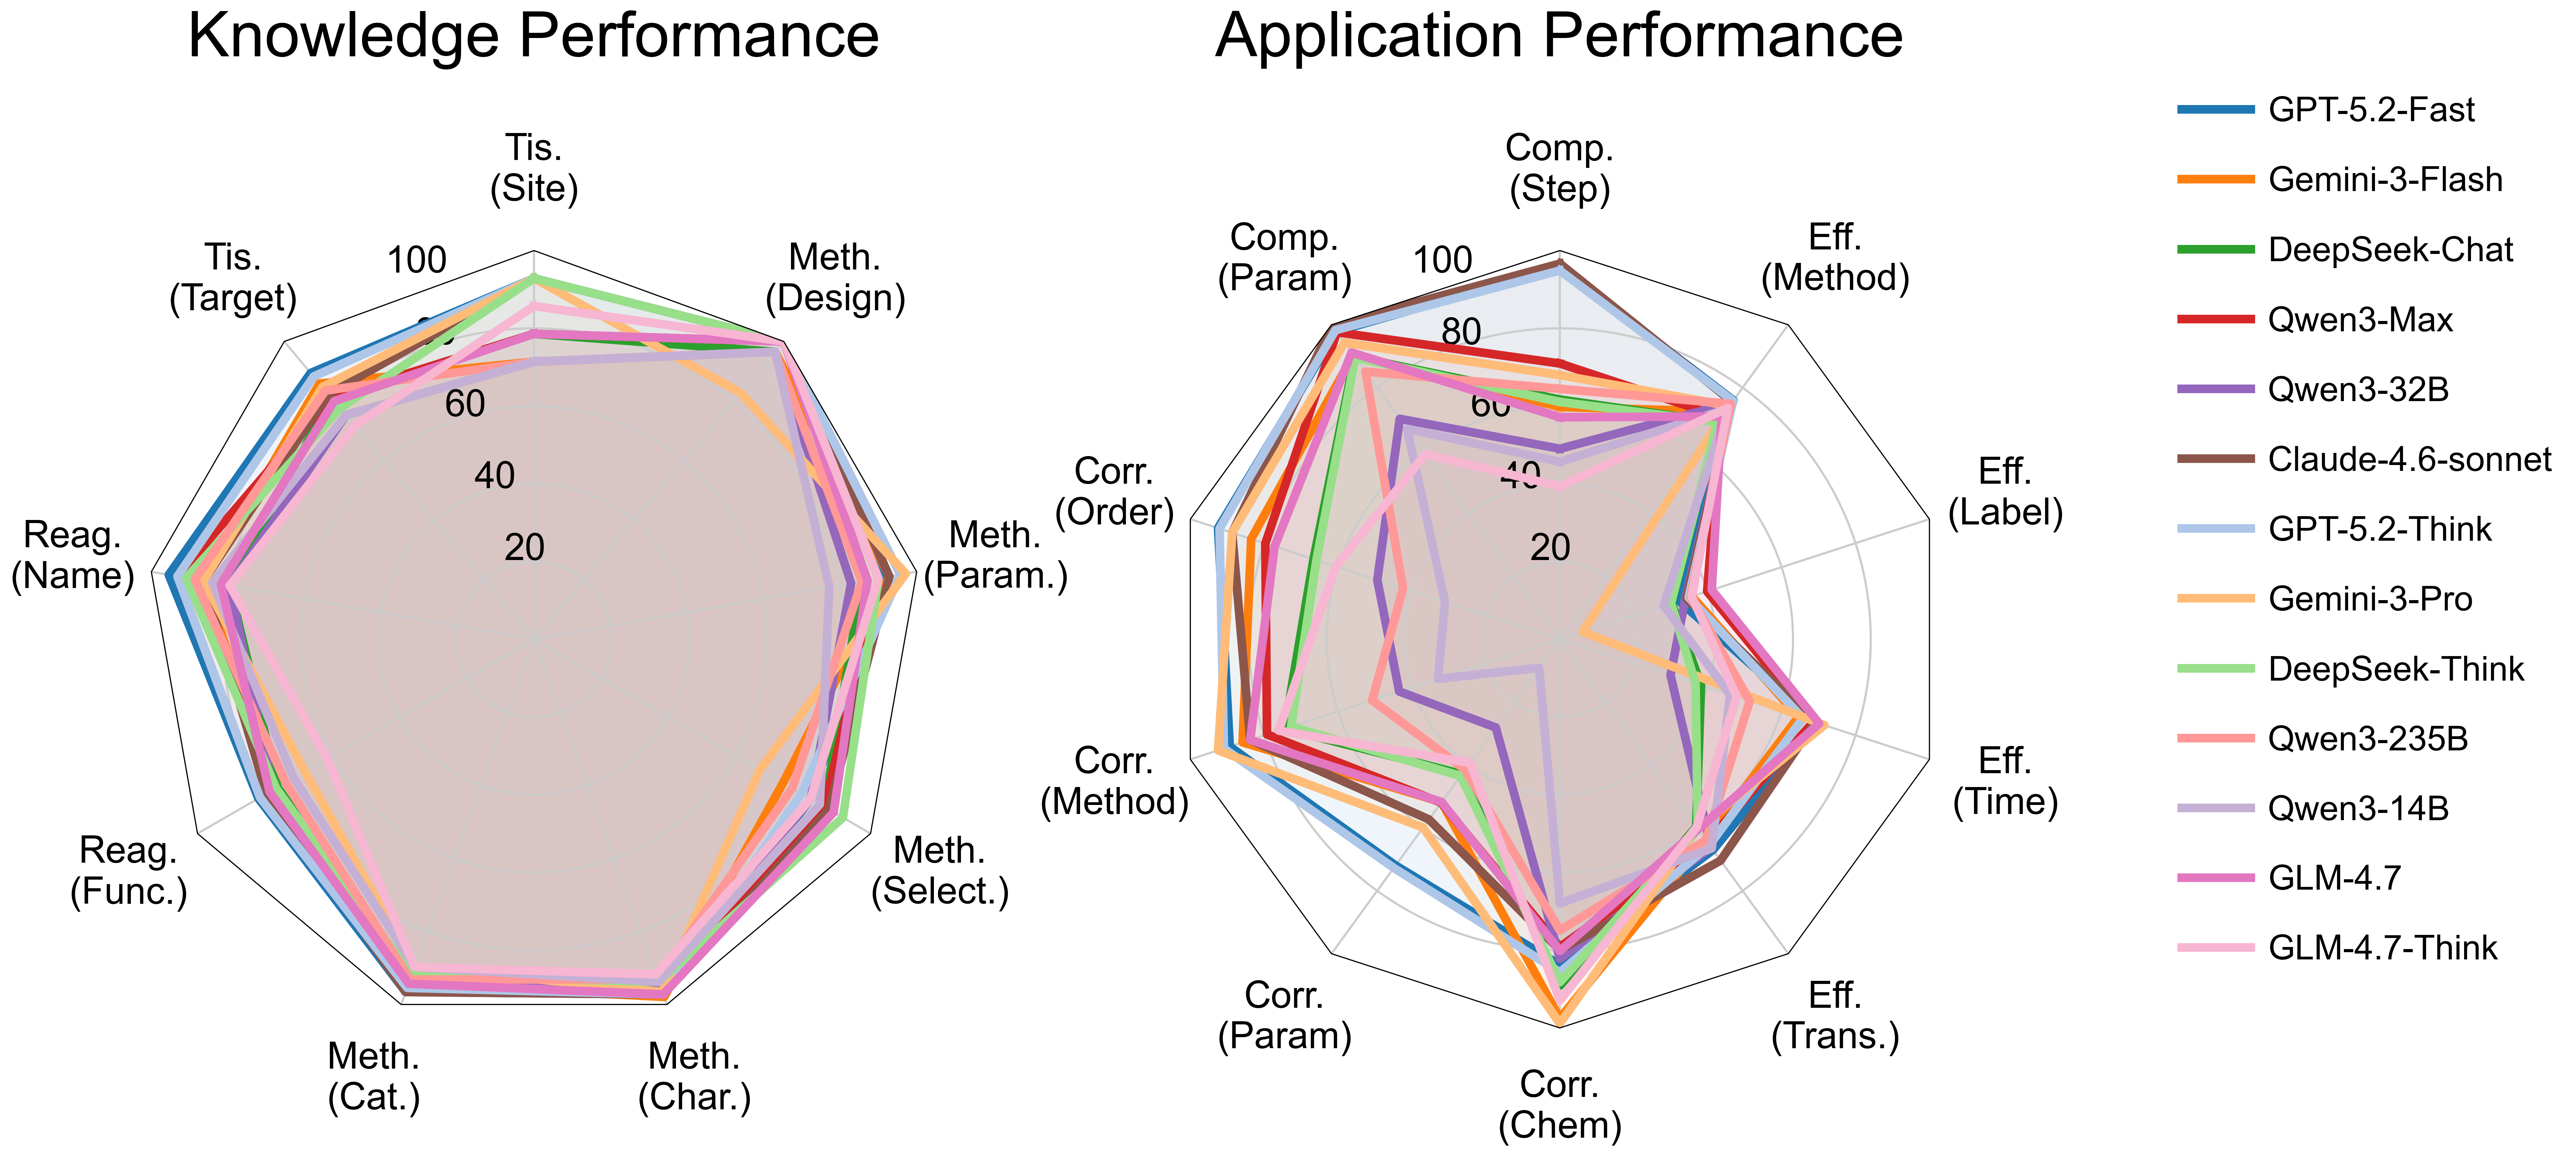
\includegraphics[width=0.62\textwidth]{figures/radar_chart.png}
    \caption{ClearEval results for 13 LLMs. Left: Knowledge Index components
    (Tissue, Reagent, Method). Right: Application dimensions and sub-scores.
    Knowledge profiles are close across models, while Application scores show
    larger differences.}
    \label{fig:radar_chart}
\end{figure*}

\subsection{Fine-Grained Diagnosis: Where Protocols Fail}\label{sec:diag}

We examine the Effectiveness sub-scores over all 3{,}287 scored protocols.
The largest deficit is label suitability ($S_{label}$), with a mean score of
$0.32$ (Fig.~\ref{fig:violin_limits}). $S_{label}$ is computed from three
checks: marker--target match, marker--fluorophore compatibility, and
method--marker compatibility. After correction, it shows good agreement with
expert consensus (ICC $0.75$), supporting its use for failure analysis.

In total, $53\%$ of protocols receive $S_{label}=0$. Among these zero-score
cases, $86\%$ involve marker--target mismatch. These cases may also include
other labeling errors, because the categories are not mutually exclusive. The
remaining zero-score cases are mainly related to fluorophore compatibility. The
quenching-related check affects about $41\%$ of protocols and reaches zero in
about $10\%$. This shows that the main label failure is choosing a marker that
does not match the requested biological target.

Other Effectiveness terms are less impaired. RI matching ($S_{trans}$) has a
mean of $0.64$, and timing ($S_{time}$) has a mean of $0.56$. Timing errors
often occur in small-sample settings, where models over-estimate clearing time,
such as proposing about $10$ hours for a $\leq 500\,\mu$m slice that falls
within a shorter evidence-supported window. Method suitability
($S_{method}$) is higher on average (mean $0.73$) and agrees well with expert
ratings (ICC $0.82$). Thus, the main measured failure is labeling design,
especially marker--target matching, rather than clearing-method choice.

\begin{figure}[!htb]
    \centering
    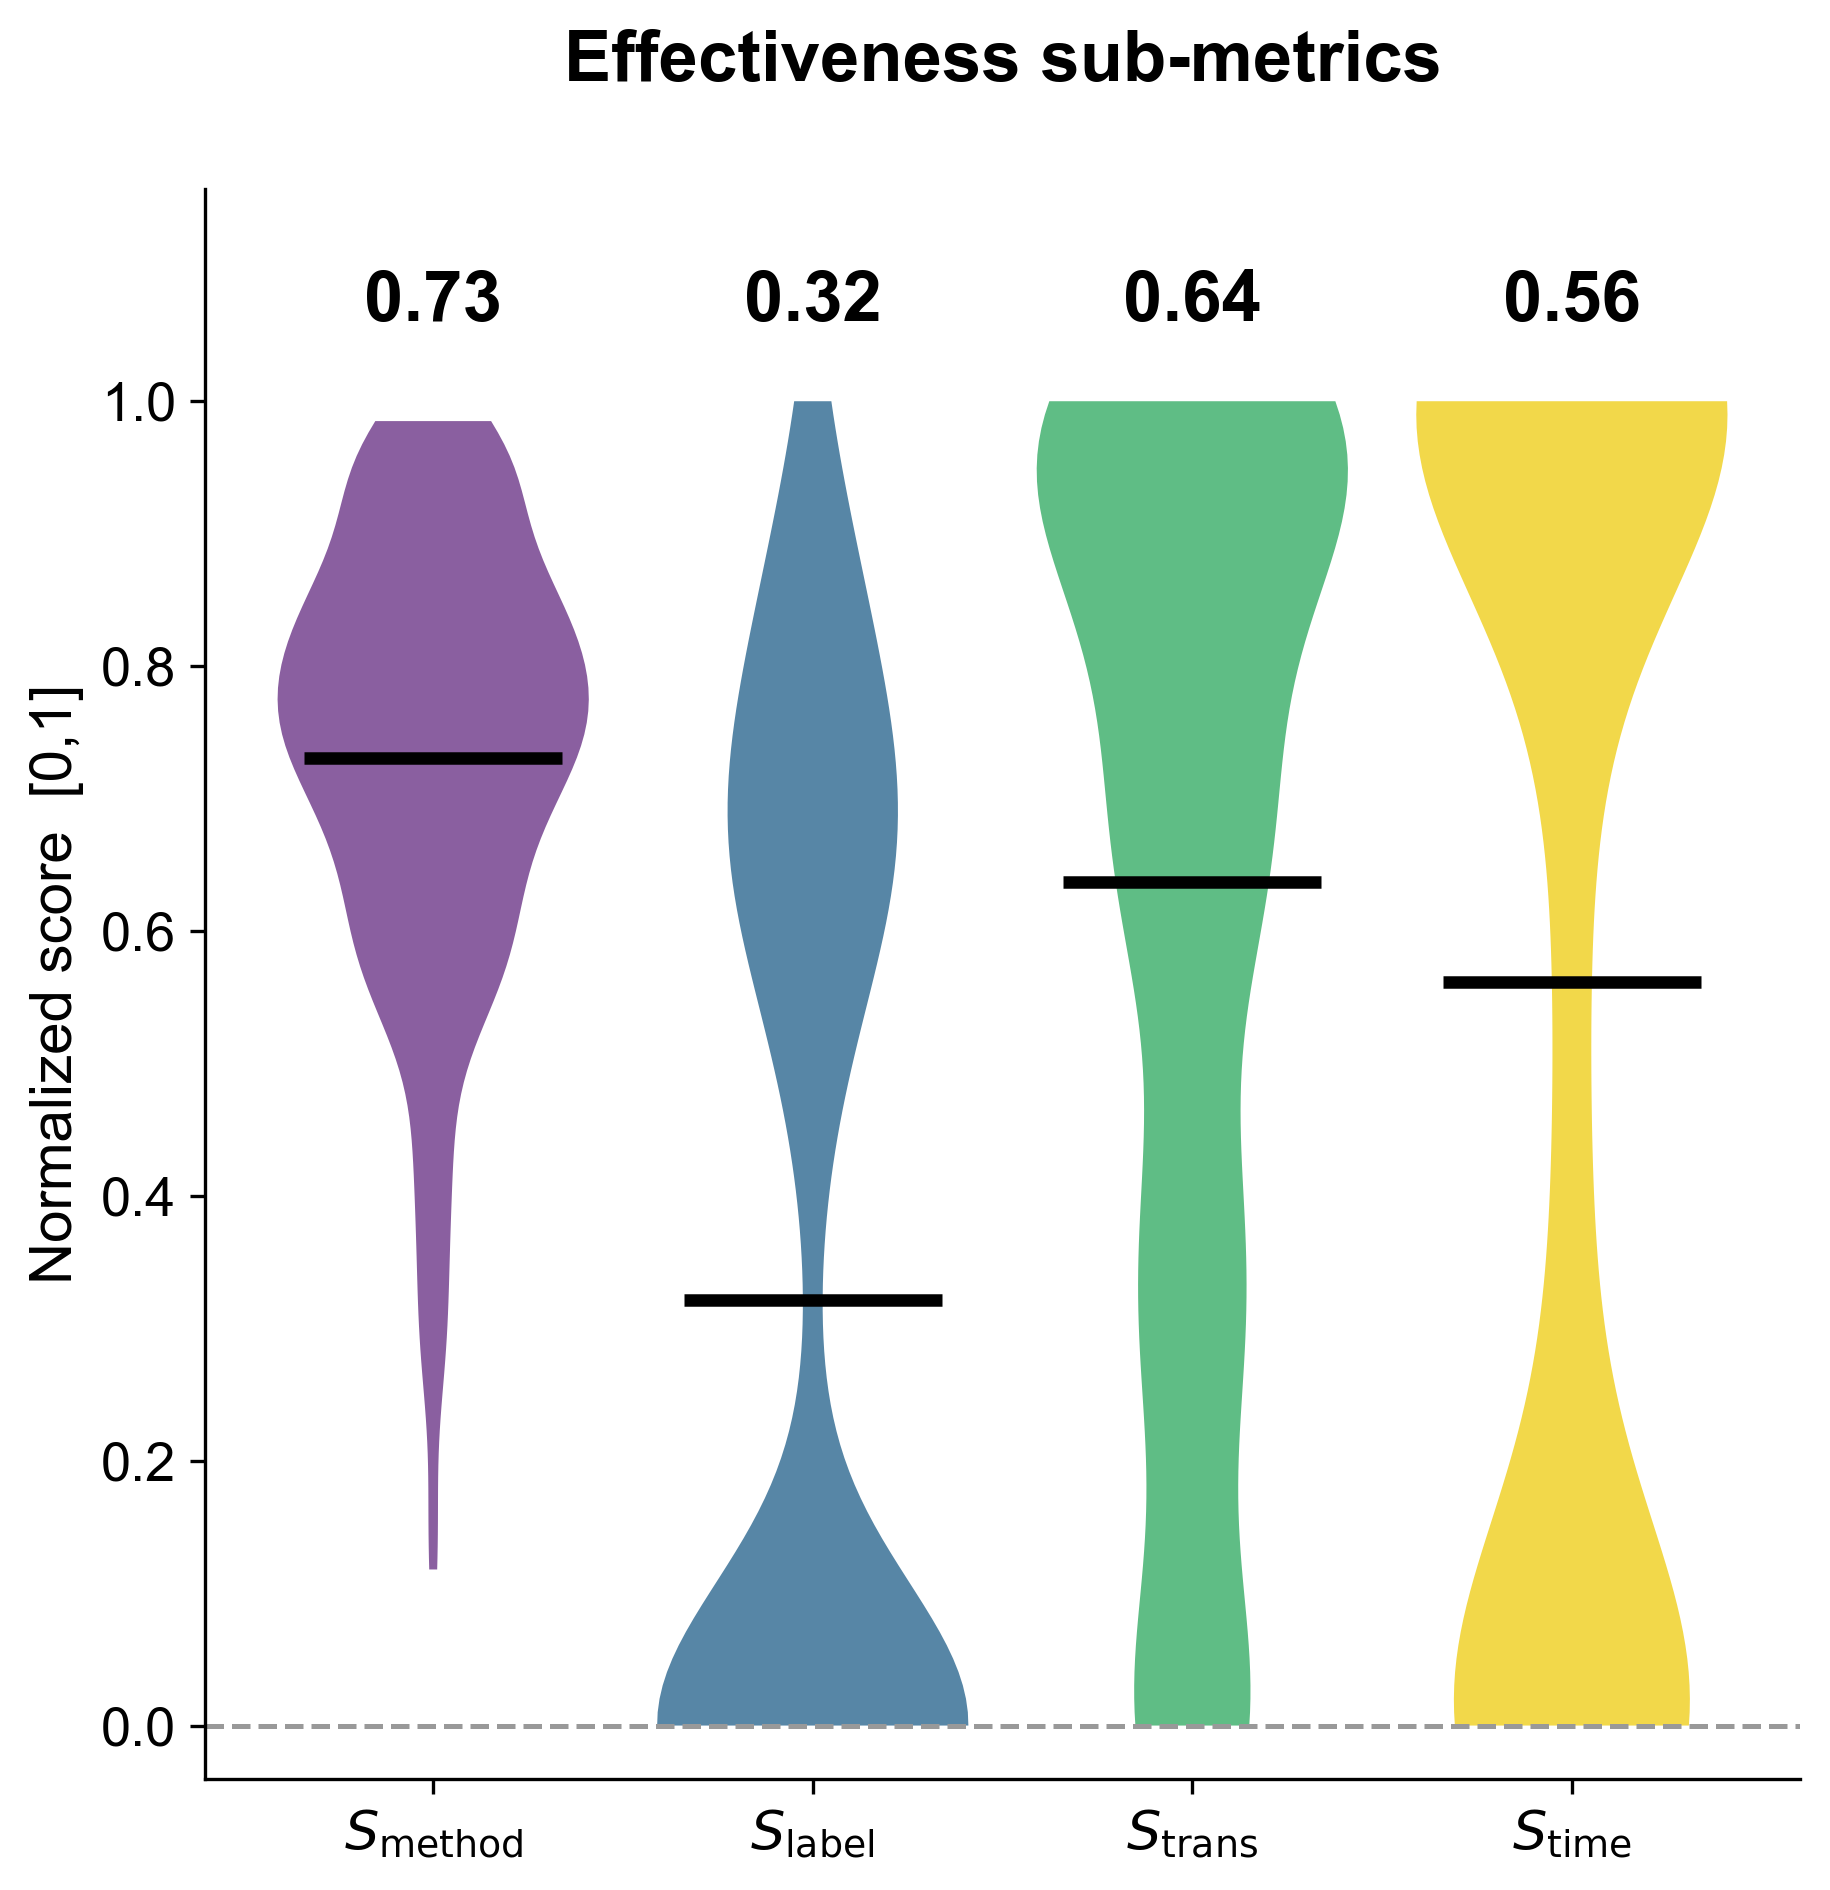
\includegraphics[width=\columnwidth]{figures/violin_plots.png}
    \caption{Effectiveness sub-score distributions over all $3{,}287$ scored
    protocols, normalized to $[0,1]$ (mean $\Diamond$, median $\circ$, IQR bar;
    $S_{method}{=}(F_{method}+1)/2$ so $0.5$ is neutral). $S_{label}$ has the
    lowest mean score ($0.32$) and agrees well with expert consensus after
    correction (ICC $0.75$). $S_{method}$ is higher on average ($0.73$) and also
    agrees well with expert ratings (ICC $0.82$).}
    \label{fig:violin_limits}
\end{figure}

\noindent\textbf{Method choice concentration.}
Model method choices are concentrated (Fig.~\ref{fig:method_usage}). iDISCO+
accounts for $43\%$ of all 3{,}287 choices, and some smaller models rely more
heavily on one clearing method. For example, Qwen3-14B selects iDISCO+ in
$74\%$ of scenarios. Choice entropy ranges from $1.35$ to $2.97$ bits across
models.

This concentration does not by itself explain the low Application scores.
iDISCO+ is broadly usable in many TOC settings, and the average $S_{method}$ is
high. Thus, method choice concentration is an observed generation pattern, but
not the main measured failure. The larger measured error is in labeling, where
models often choose markers that do not match the requested target.

\begin{figure}[!htb]
    \centering
    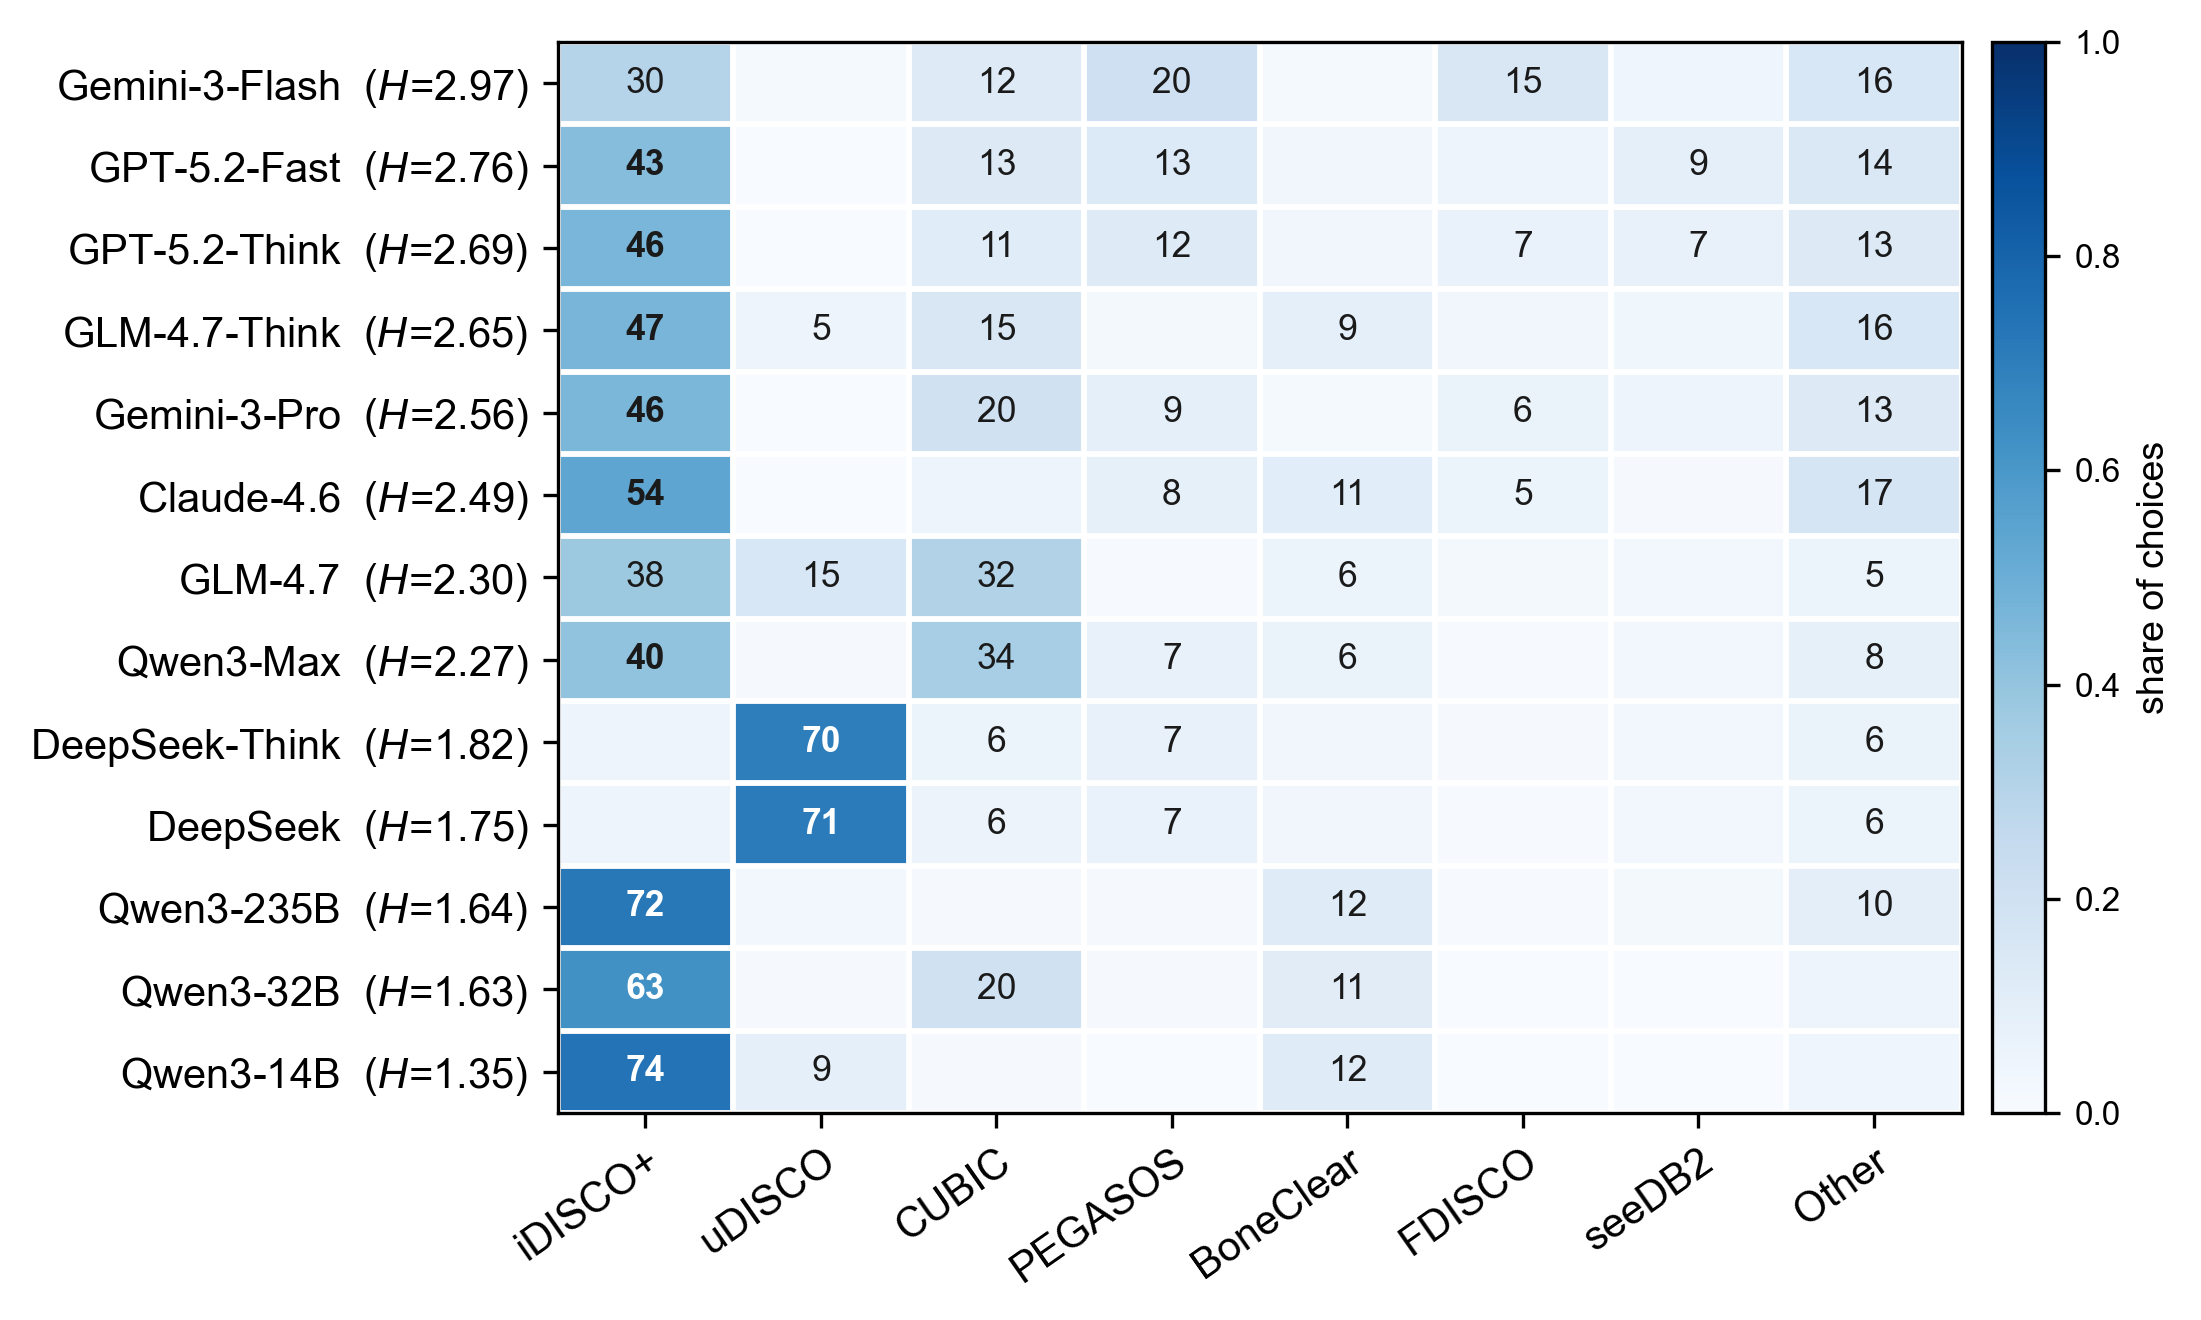
\includegraphics[width=\columnwidth]{figures/method_usage.png}
    \caption{Clearing-method choices by model, reported as percentage of generated
    protocols. Rows are sorted by choice entropy $H$. Method choices are
    concentrated in several models; iDISCO+ accounts for $43\%$ of all choices.}
    \label{fig:method_usage}
\end{figure}

\subsection{Inference-Time Grounding}\label{sec:baselines}

We test whether structured TOC grounding changes the Application results. This
experiment is not intended to cover all prompting or agent settings. It is a
controlled grounding test using the same CCE scorer as the main experiments.

We evaluate three models across the capability range: GPT-5.2-Fast, Qwen3-Max,
and Qwen3-14B. Each model is tested under three settings: the one-shot default,
one-shot with KB-RAG, and one-shot with KB-RAG plus self-check. KB-RAG prepends
a per-scenario context built from scenario metadata. The context includes
standardized scenario slots, broad target--marker guidance, and qualitative
method and compatibility records. It gives reasonable candidate ranges rather
than exact protocol answers. Gold protocols, expert scores, exact scoring
thresholds, and numeric RI/time answer keys are withheld. The same retrieved
context is used for all models. In the self-check setting, the model applies one
fixed feasibility checklist to its grounded answer and revises once.

All outputs are scored by the same calibrated CCE pipeline
(Sec.~\ref{sec:calib}), so $I_A$ is directly comparable with
Table~\ref{tab:main_results_total}. Full literature retrieval and agentic
protocol optimization are outside this controlled test.

\begin{table*}[!t]
\centering
\small
\setlength{\tabcolsep}{5pt}
\caption{Inference-time grounding on three models over 253 Application
scenarios. Com/Cor/Eff/$I_A$ are percentages. Effectiveness sub-scores are
normalized means in $[0,1]$. KB-RAG withholds gold protocols and numeric RI/time
answer keys. Self-check is one checklist-based revision.}
\label{tab:inference_time}
\begin{tabular}{llcccc cccc}
\toprule
Model & Setting & Com & Cor & Eff & $I_A$ & $S_{m}$ & $S_{lab}$ & $S_{tr}$ & $S_{ti}$ \\
\midrule
\multirow{3}{*}{GPT-5.2-Fast}
 & $1$-shot       & 97.0 & 84.4 & 61.2 & 61.2 & 0.76 & 0.32 & 0.67 & 0.70 \\
 & $+$KB-RAG      & 94.2 & 79.0 & 62.3 & 62.3 & 0.79 & 0.45 & 0.67 & 0.57 \\
 & $+$KB-RAG$+$SC & 92.0 & 80.2 & 63.2 & \textbf{63.2} & 0.79 & 0.60 & 0.60 & 0.54 \\
\midrule
\multirow{3}{*}{Qwen3-Max}
 & $1$-shot       & 87.0 & 72.5 & 60.9 & \textbf{60.9} & 0.71 & 0.40 & 0.64 & 0.69 \\
 & $+$KB-RAG      & 85.1 & 73.4 & 57.8 & 57.8 & 0.77 & 0.50 & 0.56 & 0.49 \\
 & $+$KB-RAG$+$SC & 85.2 & 73.6 & 58.6 & 58.6 & 0.76 & 0.56 & 0.57 & 0.45 \\
\midrule
\multirow{3}{*}{Qwen3-14B}
 & $1$-shot       & 58.4 & 35.3 & 53.5 & 35.3 & 0.73 & 0.28 & 0.66 & 0.46 \\
 & $+$KB-RAG      & 63.1 & 41.8 & 59.8 & 41.8 & 0.73 & 0.52 & 0.66 & 0.48 \\
 & $+$KB-RAG$+$SC & 63.3 & 42.4 & 60.6 & \textbf{42.4} & 0.73 & 0.55 & 0.66 & 0.49 \\
\bottomrule
\end{tabular}
\end{table*}

KB-RAG improves label suitability for all three models. With KB-RAG plus
self-check, $S_{label}$ increases from $0.32$ to $0.60$ for GPT-5.2-Fast, from
$0.40$ to $0.56$ for Qwen3-Max, and from $0.28$ to $0.55$ for Qwen3-14B. This
supports the diagnosis that marker--target mismatch is a major and addressable
failure mode.

The change in $I_A$ is smaller and depends on the model. KB-RAG plus self-check
improves GPT-5.2-Fast from $61.2$ to $63.2$ and Qwen3-14B from $35.3$ to
$42.4$, but Qwen3-Max decreases from $60.9$ to $58.6$. For Qwen3-Max, the label
gain is offset by lower RI and timing scores. This shows why the Application
score uses multiple feasibility checks: improving one experimental choice does
not guarantee a better full protocol.

Self-check improves over KB-RAG alone for all three models, but it does not
remove the trade-off between labeling, RI matching, and timing. Overall,
structured grounding helps with marker--target matching, while end-to-end
protocol feasibility still depends on balancing several experimental
constraints.

\noindent\textbf{Retrieval variants.}
We also tested three context designs: demand-ranked candidate methods,
RI-family-aware ranking, and RI-aware ranking with qualitative timing hints.
These variants changed different Effectiveness sub-scores. Label compatibility
improved across variants, while RI and timing scores changed with the retrieved
method context. None of the variants improved all four Effectiveness sub-scores
at the same time.

We therefore report the released, non-per-model-tuned KB-RAG setting as a
controlled grounding test. These results suggest that grounding context affects
the balance among method, labeling, RI, and timing. Joint optimization of these
choices is outside the scope of this benchmark study.

\section{Discussion and Conclusion}\label{sec:discussion}

ClearEval shows that static TOC knowledge does not reliably lead to feasible
protocol generation. In our experiments, the main measured failure is
marker--target matching in labeling design. RI matching and timing also affect
protocol feasibility. These findings support the need for protocol-level checks grounded in experimental rules, rather than evaluation based only on knowledge accuracy or text quality.

\noindent\textbf{Scope.}
ClearEval is a TOC-specific benchmark. Its claims are about TOC protocol
feasibility, not general LLM scientific competence. Applying the same approach
to another wet-lab domain would require new domain evidence, expert-reviewed
rules, and task scenarios. CCE should therefore be viewed as a re-curatable
evaluation template, not a finished multi-domain benchmark. ClearEval also
complements broad protocol benchmarks such as BioProBench~\cite{bioprobench}:
those benchmarks cover more biological areas and task types, while ClearEval
provides a deeper feasibility check within one subdomain.

\noindent\textbf{Limitations.}
ClearEval is an offline pre-experimental benchmark. It does not model all
sources of wet-lab variation, such as reagent age, batch effects, tissue
heterogeneity, or hardware differences. Its feasibility database is based on
literature, wet-lab records, and expert review, but the full parameter space is
not exhaustively re-measured. Completeness and Correctness are scored by
LLM-based rubrics, while Effectiveness is computed by non-LLM rules and
formulas. These scores are calibrated against expert consensus, but they do not
replace real wet-lab validation. The inference-time grounding experiment is a
controlled test of KB-RAG and self-check, not a full search over prompting,
retrieval, or agent settings.

Overall, ClearEval turns expert judgment on TOC protocol feasibility into
computable checks over method choice, labeling, RI matching, and timing. It
provides a depth-first feasibility benchmark for TOC and a re-curatable template
for building similar checks in other wet-lab domains.

\appendices
\section{Knowledge-Base Curation and Provenance}\label{app:curation}

\noindent\textbf{Expert review.}
The TOC feasibility database and CCE rubrics were curated with input from
tissue-clearing wet-lab experts and a knowledge-graph specialist. The review
focused on method properties, tissue and sample-scale settings, labeling
targets, marker compatibility, refractive-index matching, timing windows, and
safety-related rules.

\noindent\textbf{Knowledge bases and provenance.}
Seven JSON knowledge bases, listed in Table~\ref{tab:db_inventory}, support the
Effectiveness checks. They store method capability vectors, marker and
fluorophore compatibility, tissue and target information, RI references, timing
windows, wet-lab records, and curated literature chunks. Timing rows include a
source key, URL, evidence locator, confidence level, and review status, giving
an audit trail from each timing parameter to its evidence. Timing tolerances are
set deterministically as $\tau=0.2\times$ the median clearing time and reviewed
by experts.

\noindent\textbf{Use in scoring.}
Effectiveness is computed from protocol fields extracted from each generated
answer. $S_{method}$ uses the signed method-capability vector and the fixed
scenario-demand vector. $S_{label}$ uses marker--target, marker--fluorophore,
and method--marker compatibility rules. $S_{trans}$ uses RI references and
$\sigma_{RI}$, with unsupported method--tier pairs scored as zero. $S_{time}$
uses the evidence-supported timing window $[t_{min},t_{max}]$ and tolerance
$\tau$.

\section{Calibration Against Expert Consensus}\label{app:judge}

Table~\ref{tab:calibfull} reports the full sub-dimension agreement between
automated scores and blinded expert-consensus scores on the calibration subset
($n=240$). The LLM-judged dimensions, Completeness and Correctness, use fixed
rubrics released in the repository
(\texttt{eval\_oeq\_teacher\_rubric.txt} and
\texttt{eval\_completeness\_checklist.txt}) and are run at temperature $0.0$.
Effectiveness sub-scores are computed with non-LLM rules and formulas using the
TOC feasibility database.

The expert review for this subset was designed to produce consensus reference
scores rather than independent-rater labels. We therefore report agreement
between automated scores and expert-consensus scores, rather than human--human
inter-annotator reliability.

\begin{table}[htbp]
    \centering
    \caption{Full per-dimension agreement of automated vs.\ expert-consensus
    scores ($n{=}240$). ICC${=}$ICC(2,1); QWK${=}$quadratic-weighted $\kappa$;
    $\alpha{=}$interval Krippendorff.}
    \label{tab:calibfull}
    \small
    \begin{tabular}{l c c c c c}
        \toprule
        \textbf{Dimension} & $r$ & $\rho$ & \textbf{ICC} & \textbf{QWK} & $\boldsymbol{\alpha}$ \\
        \midrule
        $c\_step$  & 0.71 & 0.72 & 0.70 & 0.54 & 0.70 \\
        $c\_param$ & 0.71 & 0.71 & 0.68 & 0.60 & 0.67 \\
        \textbf{Completeness} & 0.77 & 0.79 & 0.75 & 0.70 & 0.75 \\
        \midrule
        $co\_order$  & 0.66 & 0.65 & 0.61 & 0.58 & 0.60 \\
        $co\_method$ & 0.83 & 0.81 & 0.79 & 0.77 & 0.79 \\
        $co\_param$  & 0.55 & 0.56 & 0.53 & 0.48 & 0.53 \\
        $co\_chem$   & 0.83 & 0.69 & 0.80 & 0.66 & 0.79 \\
        \textbf{Correctness} & 0.79 & 0.77 & 0.74 & 0.72 & 0.73 \\
        \midrule
        $S_{method}$ ($=\!(F_{method}\!+\!1)/2$) & 0.83 & 0.77 & 0.82 & 0.77 & 0.82 \\
        $S_{label}$  & 0.51 & 0.48 & 0.51 & 0.51 & 0.51 \\
        $S_{trans}$  & 0.63 & 0.46 & 0.58 & 0.52 & 0.56 \\
        $S_{time}$   & 0.80 & 0.75 & 0.78 & 0.75 & 0.78 \\
        \textbf{Effectiveness} & 0.71 & 0.72 & 0.69 & 0.68 & 0.69 \\
        \midrule
        \textbf{Overall} & 0.79 & 0.79 & 0.74 & 0.73 & 0.74 \\
        \bottomrule
    \end{tabular}
\end{table}

% ---- Bibliography ----
\bibliographystyle{IEEEtran}
\bibliography{references}

\end{document}
